\notechapter{N-20240518}{Projective Geometry as the Art of Removing Exceptions}

\section{The annoyance of parallel lines}

Euclidean geometry has a small but persistent exception: two lines meet unless they are parallel. Projective geometry removes the exception by adding points at infinity.

This is not a cosmetic choice. It changes the grammar of geometry. Statements about incidence become cleaner, and perspective drawing becomes natural.

The guiding sentence is:
\[
  \text{projective geometry sacrifices distance to save incidence.}
\]

\section{Homogeneous coordinates are ratios}

The projective line over a field \(k\) is
\[
  \mathbb P^1(k)=\{[x:y]:(x,y)\ne(0,0)\}/\sim,
\]
where
\[
  [x:y]=[\lambda x:\lambda y]\qquad(\lambda\ne0).
\]
The pair \([x:y]\) is not a point in \(k^2\). It is a line through the origin in \(k^2\).

When \(y\ne0\), the point becomes \([x/y:1]\). The missing point \([1:0]\) is the point at infinity.

Similarly,
\[
  \mathbb P^2(k)=\{[x:y:z]:(x,y,z)\ne(0,0,0)\}/\sim.
\]
The chart \(z\ne0\) is the ordinary affine plane, and the equation \(z=0\) is the line at infinity.

\section{A coordinate scene: where parallel lines meet}

The affine lines
\[
  y=0,
  \qquad
  y=1
\]
are parallel. Homogenizing them gives
\[
  y=0,
  \qquad
  y-z=0.
\]
On the line at infinity \(z=0\), both equations force \(y=0\), so the intersection is
\[
  [1:0:0].
\]
Thus projective geometry does not say that parallel lines visibly meet in the affine plane. It says that the affine plane was missing one direction point.

\begin{center}
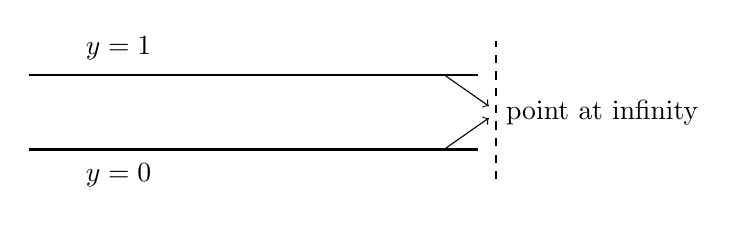
\begin{tikzpicture}[scale=0.95]
  \draw[thick] (-3,0) -- (3,0);
  \draw[thick] (-3,1) -- (3,1);
  \draw[dashed,thick] (3.25,-.4) -- (3.25,1.45);
  \node[right] at (3.25,.5) {point at infinity};
  \draw[->] (2.55,0) -- (3.15,.42);
  \draw[->] (2.55,1) -- (3.15,.58);
  \node at (-1.8,-.35) {$y=0$};
  \node at (-1.8,1.35) {$y=1$};
\end{tikzpicture}
\end{center}

The diagram is symbolic: the point at infinity is not an ordinary point far to the right. It is a direction added to complete the incidence relation.

\section{Duality: points and lines speak the same language}

A line in \(\mathbb P^2\) has equation
\[
  ax+by+cz=0.
\]
The coefficients \([a:b:c]\) are homogeneous. Thus lines themselves have projective coordinates.

Incidence is the bilinear equation
\[
  ax+by+cz=0.
\]
This symmetry produces projective duality: many theorems remain true after swapping point and line.

For instance:
\[
  \text{two points determine a line}
  \quad\longleftrightarrow\quad
  \text{two lines determine a point}.
\]
Projective geometry is full of such paired statements.

\section{Transformations and what survives}

An invertible linear map \(A:k^3\to k^3\) induces a projective transformation
\[
  [v]\longmapsto[Av].
\]
It preserves incidence but not length or angle. A circle may become an ellipse under a perspective projection, but a line remains a line.

This is the geometric lesson: once one changes the allowed transformations, one changes the invariants. Euclidean geometry cares about distances and angles. Projective geometry cares about incidence, alignment, cross-ratio, and projective equivalence.

\section{A first invariant: the cross-ratio}

For four points \(a,b,c,d\) on a projective line, the cross-ratio is written in an affine coordinate as
\[
  [a,b;c,d]
  =\frac{(c-a)(d-b)}{(c-b)(d-a)}.
\]
It is preserved by projective transformations of the line.

This formula is less important here than the role it plays. It is a warning that projective geometry is not invariant-free. It simply has different invariants from Euclidean geometry.

\section{Conics as one projective family}

A projective conic is given by a homogeneous quadratic equation
\[
  X^TAX=0,
  \qquad
  X=(x,y,z)^T.
\]
In the affine chart \(z=1\), it becomes an ordinary quadratic equation in \(x\) and \(y\). Ellipses, parabolas, and hyperbolas are different affine views of projective conics.

This explains why conics look artificially split in elementary analytic geometry. The affine chart cuts a projective object and then classifies the slice.


\section{The projective plane as all lines through the origin}

There is a concrete model that removes much of the mystery.  A point \([x:y:z]\in\mathbb P^2\) is a line through the origin in \(k^3\).  A projective line in \(\mathbb P^2\) is a plane through the origin in \(k^3\).

Then incidence becomes containment:
\[
\begin{array}{c}
  \text{projective point on projective line}\\
  \Longleftrightarrow\\
  \text{line in }k^3\text{ inside plane in }k^3.
\end{array}
\]
This model is often the easiest way to remember why two projective lines meet.  Two planes through the origin in \(k^3\) usually meet in a line through the origin, which is a projective point.

\section{Desargues as a projective-flavored theorem}

Projective geometry is naturally comfortable with theorems about incidence.  Desargues' theorem says roughly: if two triangles are perspective from a point, then the intersections of corresponding sides lie on a line.

The exact diagram is less important here than the type of statement.  It uses points lying on lines, lines meeting at points, and no measurements.  This is projective geometry's native habitat.

One reason projective geometry feels more elegant than Euclidean geometry is that many such incidence theorems survive projection.  A perspective drawing may distort lengths wildly, but it preserves collinearity and concurrence.

\section{Projective transformations in coordinates}

A projective transformation of the projective line is represented by a matrix
\[
  \begin{bmatrix}a&b\\c&d\end{bmatrix}
\]
with nonzero determinant.  In affine coordinate \(t=x/y\), it acts by a fractional linear transformation
\[
  t\longmapsto \frac{at+b}{ct+d}.
\]
This explains why the cross-ratio is built from ratios of differences: it is designed to survive these fractional linear transformations.

The point at infinity is not an exception in this formula.  It is exactly what is needed to make the transformation defined as a map of the whole projective line.

\section{The conic as a disguised projective line}

A nonsingular conic is projectively equivalent to \(\mathbb P^1\).  For example, the conic
\[
  xz-y^2=0
\]
has the parametrization
\[
  [s:t]\longmapsto [s^2:st:t^2].
\]
This formula sends a point of \(\mathbb P^1\) to a point on the conic, because
\[
  s^2t^2-(st)^2=0.
\]
So a conic is not merely a quadratic curve; projectively, it behaves like a line wrapped into the plane by quadratic coordinates.

This fact is a useful bridge to later algebraic geometry: parametrizations, homogeneous equations, and projective spaces start to work together.

The conic calculation also shows what projective completion is doing throughout the chapter.  Coordinates are replaced by ratios, missing affine directions become ordinary projective points, and the admissible transformations are exactly those that preserve incidence and cross-ratio rather than Euclidean length.
